\documentclass[letterpaper, 12pt]{article}

\usepackage{geometry}
 \geometry{
 letterpaper,
 total={170mm,257mm},
 left=20mm,
 top=20mm,
 bottom=20mm
 }
\usepackage{graphicx} % Required for inserting images
\usepackage{authblk}
\usepackage{amssymb}
\usepackage{lipsum}
\usepackage{float}
\usepackage{times}
\usepackage{amsmath}
\usepackage[format=plain,
            labelfont={bf,it},
            textfont=it]{caption}
\captionsetup{justification=raggedright,singlelinecheck=false}
\usepackage{ragged2e}
\usepackage{longtable}
\usepackage{comment}
\usepackage{setspace}
\usepackage{fancyhdr}
\usepackage{titlesec}
\usepackage[hyperindex,breaklinks]{hyperref}
\hypersetup{
    colorlinks=true,
    linkcolor=blue,
    filecolor=magenta,      
    urlcolor=blue,
    pdftitle={Overleaf Example},
    pdfpagemode=FullScreen,
    }
% \usepackage{background} % add COSIG logo to page
\usepackage[T1]{fontenc}
\usepackage{helvet}
\renewcommand{\familydefault}{\sfdefault}
\pagenumbering{gobble}
\usepackage[skip=10pt plus1pt, indent=40pt]{parskip}

\titlespacing*{\section}
{0pt}{1.5ex plus 1ex minus .2ex}{1.3ex plus .2ex}

\renewcommand\Authfont{\fontsize{12}{14.4}\selectfont}
\renewcommand\Affilfont{\fontsize{9}{10.8}\itshape}
 
\begin{document}
\flushleft

\includegraphics[width=0.5\textwidth]{img/home/241017_final_logo_mockup.png}

\section*{Tauc plots}
\addcontentsline{toc}{section}{Tauc plots}
\textit{Last updated: 25 March 2025}

In electrochemical studies, it is often necessary to estimate the \href{https://en.wikipedia.org/wiki/Band_gap}{band gap energy} of a \href{https://en.wikipedia.org/wiki/Semiconductor}{semiconducting} material. This the energy that any electron in the material must absorb in order to move from the valence band (the energy level at which electrons are bound to atoms in the material) to the conduction band (the energy level at which electrons can freely move around a material). Band gap energy is frequently estimated with a \href{https://en.wikipedia.org/wiki/Tauc_plot}{Tauc plot}, a visualization method developed by Czech-American physicist \href{https://en.wikipedia.org/wiki/Jan_Tauc}{Jan Tauc} (pronounced  ``touts'').

Tauc plots are generated by transforming the absorbance spectrum or diffuse reflectance spectrum of a material. An absorbance spectrum plots the absorbance of light passing through a material $A$ versus the wavelength of that light $\lambda$. $A$ is calculated by
\begin{equation*}
    A = \log_{10}(\frac{I_0}{I})
\end{equation*}
where $I_0$ is the intensity of light entering the material, $I$ is the intensity of light leaving the material and $A$ is expressed in arbitrary units. For example, if a material absorbs 99\% of the light passing through it at a particular wavelength, then $I = 0.01I_0$ and $A = log_{10}(\frac{I_0}{0.01I_0}) = log_{10}(100) = 2$. Absorption $A$ is related to the absorption coefficient $\alpha$ by the \href{https://en.wikipedia.org/wiki/Beer%E2%80%93Lambert_law#History}{exponential attenuation law}
\begin{equation*}
    I = I_0e^{-\alpha d}
\end{equation*}
where $d$ is the length of the path of light as it passes through the material. Rearranging this equation, we obtain
\begin{equation*}
    \log_{10}(\frac{I_0}{I}) = A = \log_{10}(e)\alpha d.
\end{equation*}
Because $d$ is typically 1 cm (absorbance spectra are usually measured by placing a solution in a cuvette 1 cm wide), this simplifies to
\begin{equation*}
    \alpha = 2.302\textrm{cm}^{-1}A.
\end{equation*}
To make a Tauc plot, one must convert $A$ to $\alpha$ and convert $\lambda$ to the energy of incident photons $h\nu$, which may be accomplished by
\begin{equation*}
    h \nu \approx 1239.8/\lambda
\end{equation*}
where $h\nu$ is expressed in electron volts (eV) and wavelength is expressed in nanometers (nm). Next, $h\nu$ is plotted on the x-axis and $(\alpha h \nu)^{1/\gamma}$ is plotted on the y-axis, where $\gamma = 1/2$ for estimating direct band gap energy and $\gamma = 2$ for estimating \href{https://www.doitpoms.ac.uk/tlplib/semiconductors/direct.php}{indirect band gap energy}.

If estimating band gap energy from a reflectance spectrum (where the reflectance $R$ of light off of the surface of a material, typically expressed as a percentage or fraction, is plotted versus the wavelength of that light $\lambda$), the y-axis instead shows $(F(R) h \nu)^{1/\gamma}$ where
\begin{equation*}
    F(R) = \frac{(1-R)^2}{2R}.
\end{equation*}
$F(R)$ is known as the \href{https://en.wikipedia.org/wiki/Kubelka%E2%80%93Munk_theory}{Kubelka-Munk function}. Note that in a Tauc plot the x-axis will always show $h\nu$ but the y-axis may show $(\alpha h \nu)^{1/\gamma}$ or $(F(R) h \nu)^{1/\gamma}$ depending on whether an absorbance or reflectance spectrum was used.

If a material does in fact have an optical band gap, the resultant Tauc plot trace should have low values on the y-axis at low energy values (i.e. the left part of the plot), followed by a steep, linear increase. This indicates that the material shows negligible absorbance and high reflectance for light energies lower than its band gap energy. The final step to estimate band gap energy is to make a linear fit to the linear region of the trace and extend this linear fit to the line $y = 0$ (i.e. $(\alpha h \nu)^{1/\gamma} = 0$, the mathematical abscissa/x-axis of the graph). The x-intercept of this linear fit (i.e. the value of $x$ where the linear fit intersects the mathematical abscissa/x-axis of the graph) is an approximation of the material's band gap energy. This is by the equation

%
\begin{equation*}
(\alpha h \nu)^{1/\gamma} = \beta(h \nu - E_g)
\end{equation*}
%
where $\beta$ is a constant.  By this equation, $h \nu = E_g$ if and only if $(\alpha h \nu)^{1/\gamma} = 0$.

\pagebreak
\begin{figure}[h!tbp]
    \centering
    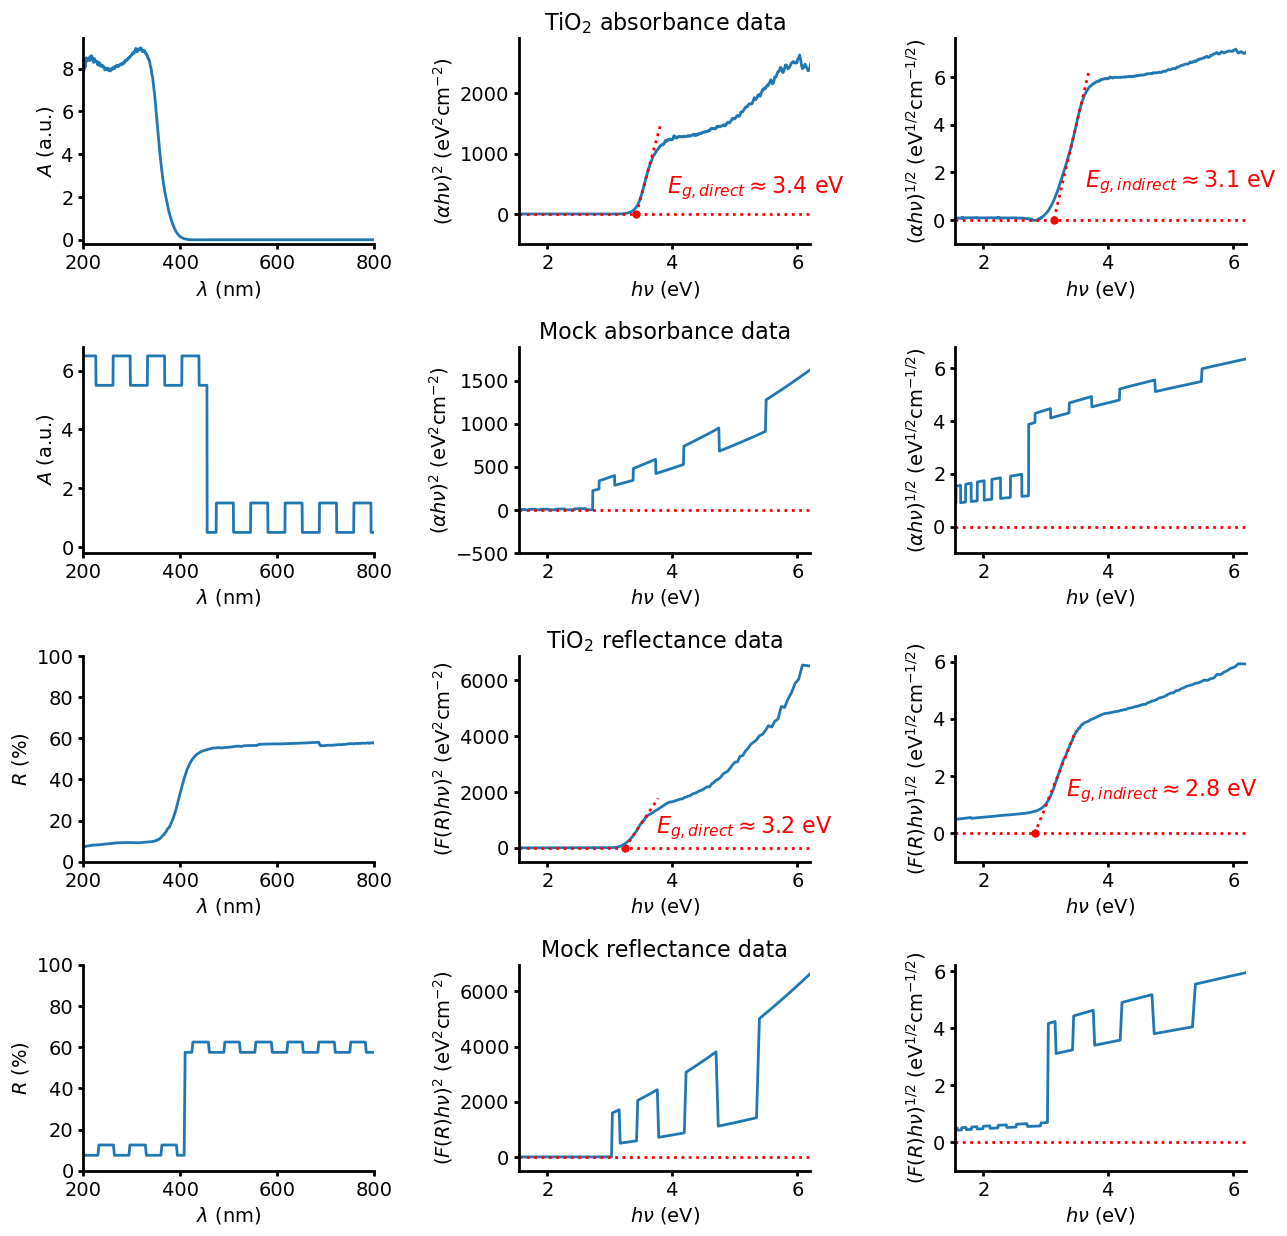
\includegraphics[width=\textwidth]{img/tauc/250320_tauc_demo.png}
    \caption*{Examples of real and mock absorbance and reflectance data and their corresponding Tauc plot transformations. For the real data, linear fits are made to the linear region of the graph and shown as red dotted lines. The intersection between this line and the abscissa of the graph (i.e. $y = 0$ or $(\alpha h \nu)^{1/\gamma} = 0$, shown as a horizontal red dotted line) gives an estimate of the material's band gap energy $E_g$. Note that although the Tauc plot interpretations of the real data shown here are methodologically sound, they likely do not yield accurate band gap energies for titanium dioxide (TiO$_2$). TiO$_2$ is semiconducting material with an \href{https://doi.org/10.1038/srep04043}{indirect band gap of 3.0 eV to 3.2 eV}. Absorbance data was shared for a Tauc plot analysis pipeline written by   \href{https://github.com/alexey-krasnov/absorption_tauc_plot}{Aleksei Krasnov}, which was used to perform Tauc transformations. Reflectance data was shared by \href{https://doi.org/10.5281/zenodo.14608640}{Polina et al (2025)}.}
\end{figure}

When analyzing a composite material (perhaps made of two semiconducting materials with different band gap energies), it is common to make two linear fits: one to the steep linear rise in the curve and one to the slope immediately preceding it as a baseline. The band gap is then estimated as the x-value of the intersection point of these two linear fits. This ``simplified'' procedure is described by \href{https://doi.org/10.1021/acs.jpclett.8b02892}{Maku\l{}a et al. (2018)} and demonstrated in Example 2 below.

Note that the Tauc plot is not the only method for estimating band gap energy. \href{https://doi.org/10.1016/j.apmt.2024.102094}{Andrade et al. (2024)} describe various methods, such as the Cody method/plot, the Boltzmann method/regression and the Kramers-Kronig method/regression/transformation.

It is common mistake to calculate $E_g$ not from the intercept of the linear fit with the line $(\alpha h \nu)^{1/\gamma} = 0$, but instead from the intercept of the linear fit with the line $(\alpha h \nu)^{1/\gamma} = y_{\rm min}$, where $y_{\rm min}$ is the bottom limit of the y-axis as plotted (i.e. where the x-axis \textit{appears} on the graph instead of at $y =0$). If $y_{\rm min} < 0$, this results in the band gap energy being underestimated. If $y_{\rm min} > 0$, this results in the band gap energy being overestimated.

Linear fits are also frequently made arbitrarily to regions of the trace other than the steep linear portion (such as to the ``elbow'' of the curve), rendering highly inaccurate estimates for band gap energy.

\subsection*{Example 1: Correct application of Tauc plot procedure}

\href{https://doi.org/10.1021/acs.jpclett.8b02892}{Maku\l{}a et al. (2018)} describe how to correctly apply the Tauc plot method and provide several examples.

\begin{figure}[h!tbp]
    \centering
    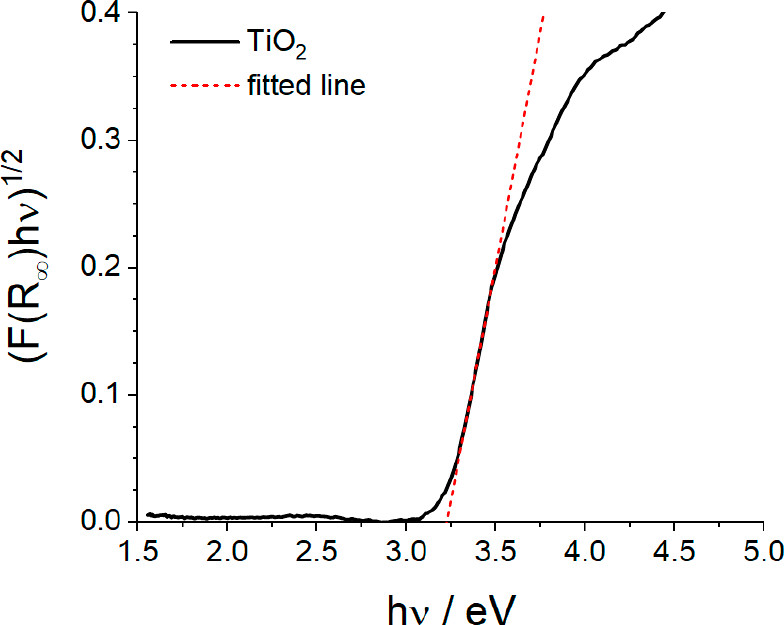
\includegraphics[width=0.6\textwidth]{img/tauc/images_large_jz-2018-02892b_0001.jpeg}
    \caption*{Tauc plot for TiO$_2$ showing the appropriate application of the Tauc plot for bang gap energy determination. Adapted from Figure 1 of \href{https://doi.org/10.1021/acs.jpclett.8b02892}{Maku\l{}a et al. (2018)}.}
\end{figure}

\pagebreak

\subsection*{Example 2: Correct application of Tauc plot procedure with baseline fitting}

\begin{figure}[h!tbp]
    \centering
    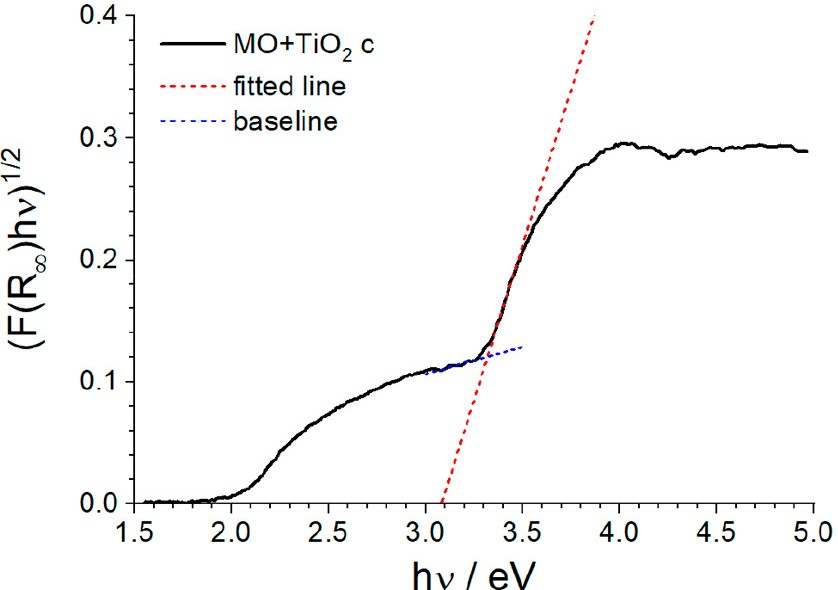
\includegraphics[width=0.6\textwidth]{img/tauc/images_large_jz-2018-02892b_0004.jpeg}
    \caption*{Tauc plot for a mixture of methyl orange (MO) dye and TiO$_2$ showing the appropriate application of the Tauc plot for bang gap energy determination with a baseline correction. Adapted from Figure 4A of \href{https://doi.org/10.1021/acs.jpclett.8b02892}{Maku\l{}a et al. (2018)}.}
\end{figure}

\subsection*{Example 3: Problematic band gap determination via Tauc plot}

\href{https://doi.org/10.1002/pssa.202200734}{Saleem et al. (2023)} report on the synthesis and characterization of a MnS and reduced graphene oxide (rGO) nanocomposite photocatalytic degradation of methylene blue dye. The article's Tauc plots contain many errors that directly compromise the authors' estimation of band gap energy:

\begin{itemize}
    \setlength\itemsep{-0.5em}
    \item Linear fits are not made to the linear portions of the curve.
    \item Band gap energy is estimated at the intersection of the linear fit and where the x-axis appears on the graph, not actually at the line $y = 0$. In two graphs, the intercept is evaluated below $y = 0$ and in another the intercept is evaluated above $y = 0$.
    \item The y-axis is labeled ``$\alpha h \nu$ (eVcm$^{-1}$)'', which does not correspond to a direct or indirect transition.
\end{itemize}

The article was retracted in 2025 with the retraction notice stating that the ``retraction has been agreed following an investigation into concerns raised by a third party, which revealed inconsistencies in the Tauc plots shown in Figure 4 [...] In view of the substantial problems with the Tauc plots and additional inconsistencies in other data presented, severe doubts about the reliability of the data remain''.

\begin{figure}[h!tbp]
    \centering
    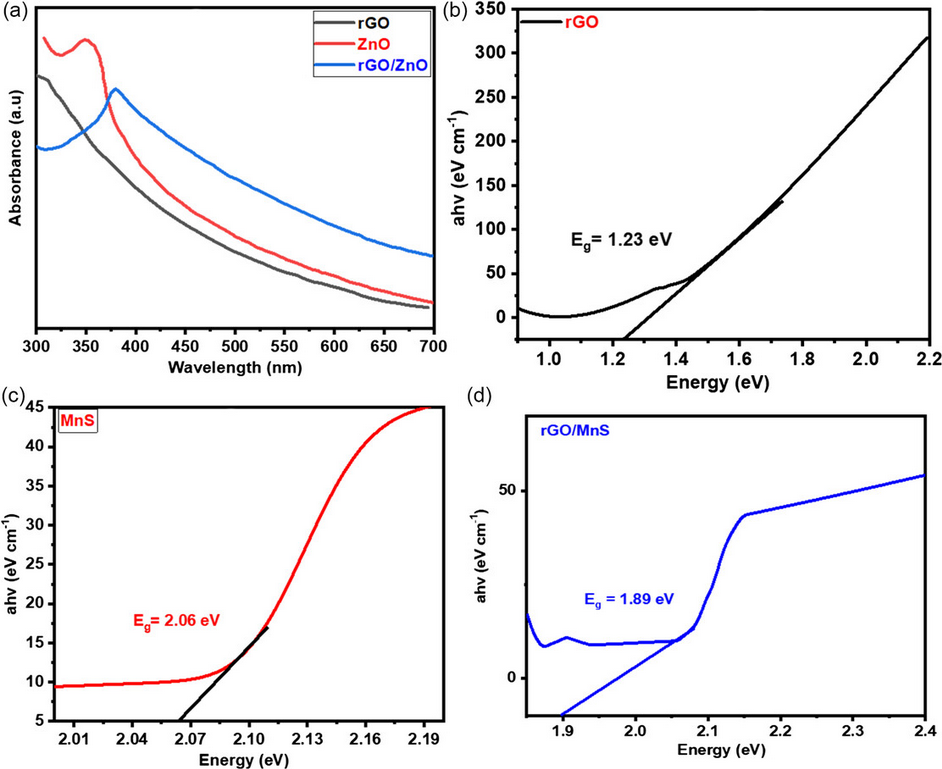
\includegraphics[width=\textwidth]{img/tauc/image-1719173331222.png}
    \caption*{Absorbance spectra and their corresponding problematic Tauc plots, adapted from Figure 4 of \href{https://doi.org/10.1002/pssa.202200734}{Saleem et al. (2023)}. In the Tauc plot for rGO shown in panel b, the band gap energy is evaluated at $y \sim -25$. In the Tauc plot for MnS shown in panel c, the linear fit is made arbitrarily to the ``elbow'' of the curve and the band gap energy is evaluated at $y \sim 5$. In the Tauc plot for rGO/MnS shown in panel d, the linear fit is made arbitrarily to the ``elbow'' of the curve and the band gap energy is evaluated at $y \sim -10$. In all Tauc plots shown, the y-axis is labeled ``$\alpha h \nu$ (eVcm$^{-1}$)'', which does not correspond to a direct or indirect transition. Finally, it is unclear that these Tauc plots actually correspond to the absorbance spectra shown in panel a (for instance, the Tauc plot for rGO/MnS indicates that there should be a ``kink'' in the absorbance spectrum for rGO/MnS around 1.85 eV / 670 nm that is absent in panel a). These factors result in unreliable estimates of band gap energy.}
\end{figure}

\pagebreak

\subsection*{Example 4: Problematic band gap determination via Tauc plot yields opposite conclusions}

\href{https://doi.org/10.1007/s10948-020-05735-4}{Arshad et al. (2020)} report on the synthesis of nanoferrites with various doping concentrations of copper. In the article's Tauc plots, the band gap energy is evaluated for each material at the intersection of the linear fit with the line $(\alpha h \nu)^{2} = -25$, the bounding box of the graph, not $(\alpha h \nu)^{2} = 0$, the graph's actual abscissa. Evaluating each material's band gap energy correctly would lead the authors to conclude that band gap energy increases with increasing copper concentration. Instead, the authors severely underestimate band gap energy and come to the opposite conclusion: that band gap energy decreases with increasing copper concentration.

\begin{figure}[h!tbp]
    \centering
    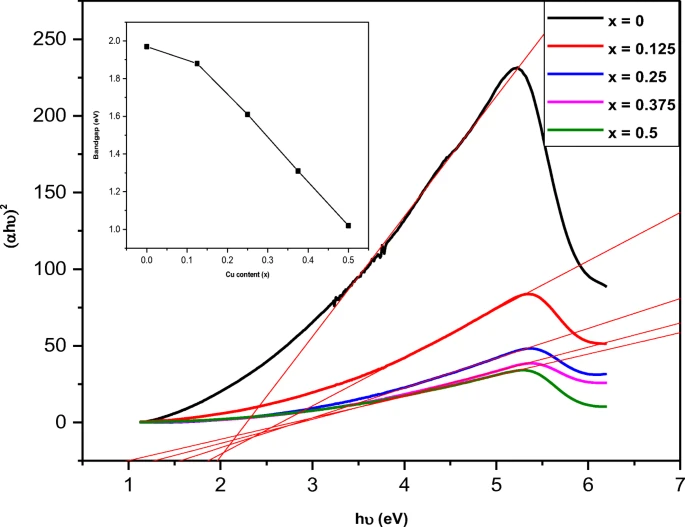
\includegraphics[width=\textwidth]{img/tauc/image-1733426799694.png}
    \caption*{Problematic Tauc plots adapted from Figure 5 of \href{https://doi.org/10.1007/s10948-020-05735-4}{Arshad et al. (2020)}.}
\end{figure}

\pagebreak
\subsection*{Example 5: Arbitrary linear fit}

\href{https://doi.org/10.1021/acsami.3c08470}{Yan et al. (2023)} report on the synthesis of metal-organic frameworks and tuning their electrical properties via metal substitution. In the Tauc plot shown for Cu-MOF-5, the authors arbitrarily make the linear fit to the ``elbow'' of the curve, resulting in a severe underestimation of band gap energy for the material. This arbitrary fit produces a band gap energy estimate that matches the results of the authors' density functional theory (DFT) simulations.

\begin{figure}[h!tbp]
    \centering
    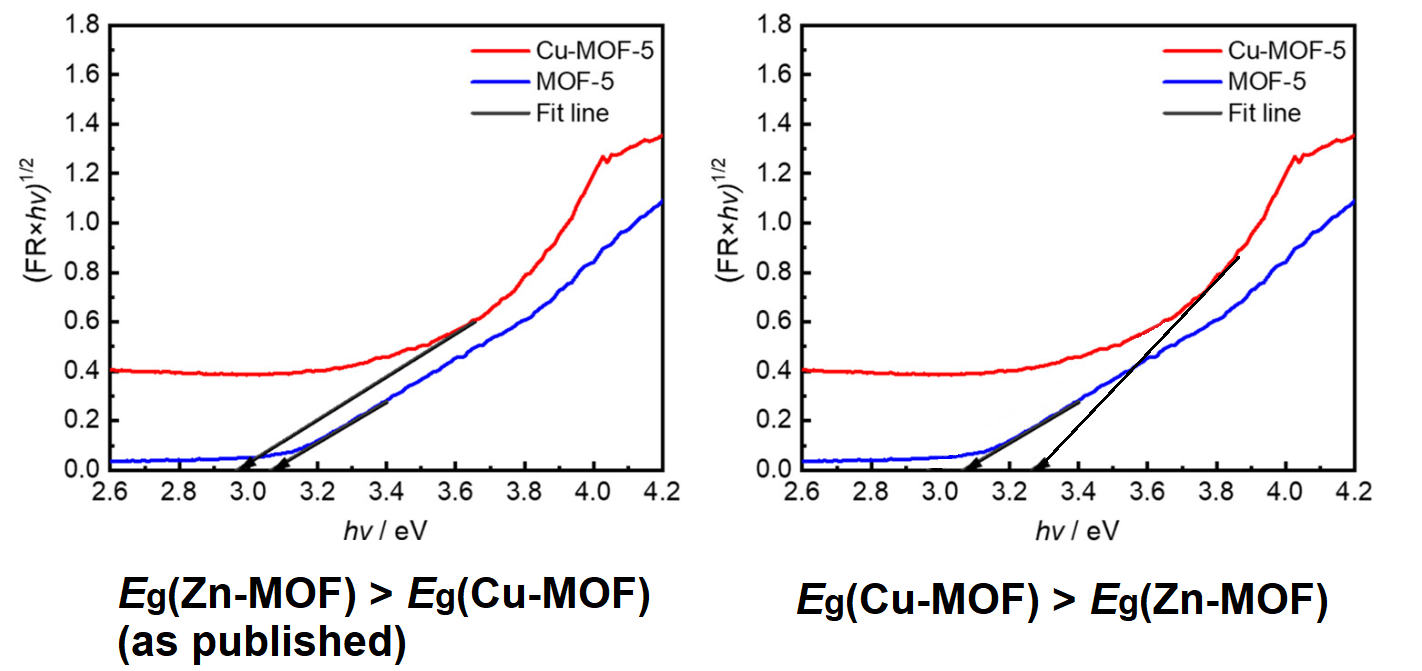
\includegraphics[width=\textwidth]{img/tauc/image-1736207336000.png}
    \caption*{Problematic Tauc plots adapted from Figure 6 of \href{https://doi.org/10.1021/acsami.3c08470}{Yan et al. (2023)} by \href{https://pubpeer.com/publications/7EBEC9D9FBC9A017CB258235844AB5\#3}{Sylvain Bern\'es}. As shown in the right panel, if linear fits are made arbitrarily to the curve, the band gap energy for Cu-MOF-5 can be alternatively interpreted as higher or lower than that of MOF-5.}
\end{figure}

\pagebreak

\subsection*{Example 6: Wrong transformation, wrong axis}

\href{https://doi.org/10.1016/j.optmat.2014.06.033}{Mhareb et al. (2014)} report on changes to the optical properties of borate glasses doped with neodymium ions. The Tauc plot shown in Figure 4 is supposed to represent indirect transitions. However, the y-axis shows a transform of $(\alpha h \nu)^{2}$, which is for direct transitions, while indirect transitions would use a transform of $(\alpha h \nu)^{1/2}$. Further, for this Tauc plot, the band gap energy is evaluated at the intersection of the linear fit with the line $(\alpha h \nu)^{2} = -1000$, the bounding box of the graph, not $(\alpha h \nu)^{2} = 0$, the graph's actual abscissa.

\begin{figure}[h!tbp]
    \centering
    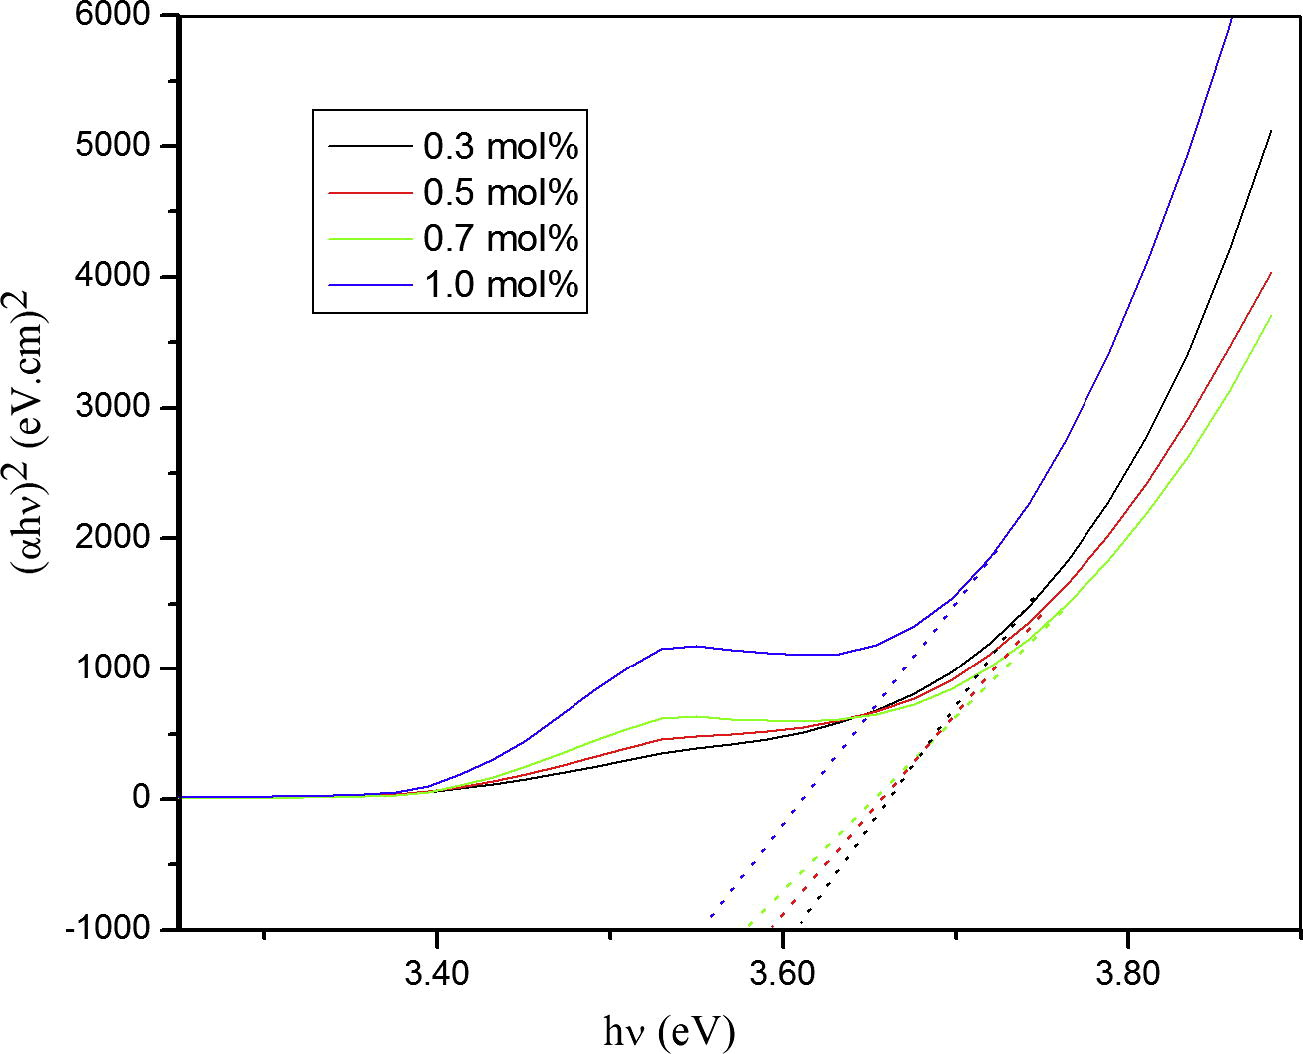
\includegraphics[width=0.6\textwidth]{img/tauc/1-s2.0-S0925346714003255-gr5_lrg.jpg}
    \caption*{Problematic Tauc plot adapted from Figure 5 of \href{https://doi.org/10.1016/j.optmat.2014.06.033}{Mhareb et al. (2014)}.}
\end{figure}

\subsection*{Additional resources}

\begin{itemize}
    \setlength\itemsep{-0.5em}
    \item \href{https://doi.org/10.1021/acs.jpclett.8b02892}{``How To Correctly Determine the Band Gap Energy of Modified Semiconductor Photocatalysts Based on UV–Vis Spectra'' (2018)}
    \item \href{https://doi.org/10.1016/j.jssc.2016.05.010}{``Direct optical band gap measurement in polycrystalline semiconductors: A critical look at the Tauc method'' (2016)}
    \item \href{https://doi.org/10.1002/adfm.202304523}{``Limitations of the Tauc Plot Method'' (2023)}
    \item \href{https://gepac.github.io/2019-06-07-projeto-bandGap/}{``C\'alculo de Band-gap com Python'' (2019, Portuguese)}
    \item \href{https://github.com/alexey-krasnov/absorption_tauc_plot}{GitHub: absoprtion\_tauc\_plot}
    \item \href{https://github.com/LiamWilbraham/taucauto}{GitHub: taucauto}
\end{itemize}

\end{document}